\documentclass[a4paper]{article}

\usepackage[margin=2.5cm]{geometry}
\usepackage[pdftex]{graphicx}
\usepackage[utf8]{inputenc}
\usepackage[T1]{fontenc}
\usepackage{textcomp}
\usepackage{babel}
\usepackage{amsmath, amssymb}
\usepackage[colorlinks=true,linkcolor=blue]{hyperref}
\usepackage{float}
\usepackage{mathrsfs}
%\usepackage{enumitem}
%% for identity function 1:
%\usepackage{bbm}
%%For category theory diagrams:
%\usepackage{tikz-cd}
%%For code (e.g. python) in latex:
%\usepackage{listings}
%
%Usage: 
%\begin{lstlisting}[language=Python]
%\end{lstlisting}

\newcommand{\incfig}[2][1]{%
\def\svgwidth{#1\columnwidth}
\import{./figures/}{#2.pdf_tex}
}


% figure support
\usepackage{import}
\usepackage{xifthen}
\pdfminorversion=7
\usepackage{pdfpages}
\usepackage{transparent}

\pdfsuppresswarningpagegroup=1

\setlength\parindent{0pt}

\newcommand{\qed}{\tag*{$\blacksquare$}}
\newcommand{\qedwhite}{\hfill \ensuremath{\Box}}

%Inequalities
\newcommand{\cycsum}{\sum_{\mathrm{cyc}}}
\newcommand{\symsum}{\sum_{\mathrm{sym}}}
\newcommand{\cycprod}{\prod_{\mathrm{cyc}}}
\newcommand{\symprod}{\prod_{\mathrm{sym}}}

%Linear Algebra

%Redeclaring Span and image
\DeclareMathOperator{\Span}{span}
\DeclareMathOperator{\Ima}{Im}
\DeclareMathOperator{\diag}{diag}
\DeclareMathOperator{\Ker}{Ker}
\DeclareMathOperator{\ob}{ob}


%Row operations
\newcommand{\elem}[1]{% elementary operations
\xrightarrow{\substack{#1}}%
}

\newcommand{\lelem}[1]{% elementary operations (left alignment)
\xrightarrow{\begin{subarray}{l}#1\end{subarray}}%
}

%SS
\DeclareMathOperator{\supp}{supp}
\DeclareMathOperator{\Var}{Var}

%NT
\DeclareMathOperator{\ord}{ord}

%Alg
\DeclareMathOperator{\Rad}{Rad}
\DeclareMathOperator{\Jac}{Jac}

\DeclareMathAlphabet{\pazocal}{OMS}{zplm}{m}{n}
\newcommand{\unif}{\pazocal{U}}

\begin{document}
    \textbf{1:}\\
    (a,b) First we show $\varphi$ is surjective: let $(z,w) \in Y$. Then
    $z^3 - w^2 = 0$ so $z^3 = w^2$. Then
    $ \varphi (\sqrt{z}) = \left( z, z^{\frac{3}{2}} \right) =
    \left( z, \left( z^3 \right)^{\frac{1}{2}} \right) = \left( z,
    w \right)  $. Thus $\varphi$ is surjective.\\
    \linebreak
    Assume $\varphi(z) = \varphi(w)$. Then
    $\left( z^2 , z^3 \right) = \left( w^2, w^3 \right) $. Thus
    $z = \pm w$. If $z = -w$, then $w^3 = z^3 = (-w)^3 = -w^3$ and thus $w
    = 0$, but then $z = -w = 0$ so $(z,w) = (0,0)$. So  $\varphi$ is
    injective.\\
    \linebreak





    Now define 
    $\psi  \colon k [x,y] \to k[t]$ by $\psi(x) = t^2, \psi (y) = t^3$ with $k
    = \mathbb{C}$. We claim $\Ker \psi = \left( x^3 - y^2 \right)$.\\
    $(\supset )$ : Since $\psi$ is a homomorphism, we have
    \[
    \psi (x^3 - y^2) = \left( t^2 \right)^{3} - \left( t^3 \right)^2
    = 0.
    \] 
    $\left( \subset  \right) $ : Let $f \in \Ker \psi$. Thus $f(t^2, t^3)
    = 0$.\\
    Now since $f \in k\left[ x,y \right] = k\left[ y \right] [x] $, and $y^2
    - x^3$ is monic in $y$, we can write
    $f(x,y) = (x^3 - y^2) g + r$ where $g,r \in k\left[ x,y \right] $ 
    and $r = r_0 + y r_1$ with $r_0, r_1 \in k\left[ x \right] $. Now
    since  $0 = f(t^2 , t^3) = r_0 (t^2) + t^3 r_1(t^2)$.
    Since the degree of $t$ in $r_0(t^2)$ is even while it is odd in
    $t^3 r_1(t^2)$, we find $r_0 (t^2) = 0$ and $r_1 (t^2) = 0$ for all
    $t \in k$, so $r_0, r_1 = 0$ as they must be constant $0$ by problem 1.8 in
    Fulton.\\
    Therefore $x^3 - y^2 | f$ and so $\Ker \psi \subset \left( x^3 - y^2
    \right) $.\\
    \linebreak
    This furthermore gives us that
    $k\left[ x,y \right] / \left( x^3 - y^2 \right) \cong \Ima \psi \subset
    k\left[ x \right]  $. Now, 
    clearly $t \not\in \Ima \psi$, so in particular,
    $k\left[ x,y \right] / (x^3 - y^2) \not \cong k\left[ x \right] $.\\
    By the lemma on lecture $8$, we thus have
    that $Y$ is not isomorphic to $\mathbb{A}^{1}$.\\ 
    This shows (b), and since if $\varphi$ were an isomorphism, it
    would by the lemma induce and isomorphism of 
    $k\left[ x,y \right] / (x^3-y^2)$ with $k\left[ x \right] $, we 
    also have that $\varphi$ is not an isomorphism, completing (a).\\
    \linebreak
    
    
    (c)

     \begin{figure}[h]
         \centering
         
\includegraphics[width=0.3\textwidth]{1c.jpg}
         \label{fig:1c-jpg}
     \end{figure}
     We notice there is a kink at $(0,0)$, so it is not differentiable there.\\

     (d) $\varphi^{*} (x) (t) = x \circ \varphi (t) = t^2$ and
     $\varphi^{*}(y) (t) = y \circ \varphi(t) = t^3$, so
     $\varphi^{*}  \colon \Gamma (Y) = k\left[ x,y \right] / (x^3 - y^2) \to 
     k \left[ t \right]  = \Gamma \left( \mathbb{A}^{1} \right) $ is given by
     $x \to t^2$ and $y \to t^3$. Now
     for $f = 3x^2 + y + 5$, we have
     \[
     \varphi^{*}\overline{f} = \varphi^{*}\overline{f} (t)= f \circ \varphi (t) = 
     3 (t^2)^2 + t^3 + 5 = 3 t^{4} + t^3 + 5.
     \] 
     
     \textbf{2:}\\
     (a) We have $\varphi^{*} (x) (t) = (x) \left( \varphi(t) \right) 
     = x \left( t^2 - 1, t \left( t^2 -1 \right)  \right) = t^2 - 1$ and
     $\varphi^{*}(y) (t) = (y) (\varphi(t))
     = t \left( t^2 - 1 \right) $. 
     So for $\varphi^{*}  \colon 
     k\left[ x,y \right] = \Gamma \left( \mathbb{A}^2 \right) \to 
     \Gamma \left( \mathbb{A}^{1} \right) = k\left[ t \right] $, we have
     $\varphi^{*}(x) = t^2 - 1$ and $\varphi^{*}(y) = t \left( t^2 -1 \right)
     $.\\
     \linebreak
     (b) 
     $\varphi^{-1} \left( V(y) \right) 
     = \varphi^{-1}\left( \left\{ (x,0)  \mid x \in \mathbb{C} \right\}  \right)
     = \left\{ t \in \mathbb{C}  \mid t \left( t^2 -1 \right) = 0 \right\} 
     = \left\{ 0, 1, -1 \right\} $.\\
     \linebreak
     (c) Let $Y = V\left( y^2 - x^2 (x+1) \right) \subset \mathbb{A}^2$.\\
     We first show that $\varphi$ is surjective: 
     let $(x,y) \in Y$. Thus $y^2 = x^2 (x+1)$. Assume $x \neq 0$. Then
     $\varphi (\frac{y}{x}) = \left( \frac{y^2}{x^2} - 1,
     \frac{y}{x} \left( \frac{y^2}{x^2}-1 \right)  \right) 
     = \left( \left( x+1 \right) -1 , \frac{y}{x} \left( x+1-1 \right)  \right) 
     = \left( x,y \right) $ where the second to last equality follows since
     $\frac{y^2}{x^2} = x+1$ in $Y$.\\
     If $x = 0$, then since $y^2 = x^2 (x+1) = 0$ in $Y$, we have $y = 0$. And
     so $\varphi (1) = (0,0) = (x,y)$.\\
     Thus $\varphi$ is surjective.\\
     \linebreak
     Now assume $\varphi(t) = \varphi(s)$.
     Then
     $\left( t^2 -1, t\left( t^2 -1 \right)  \right) = \left( s^2 -1, s \left(
     s^2 -1\right)  \right) $, hence $s = \pm t$ from the first coordinate, and
     if $s = -t$, we get from the second coordinate that
     $t \left( t^2 -1 \right) = s \left( s^2 -1 \right) 
     = (-t) \left( (-t)^2 -1  \right) = - t \left( t^2 -1 \right) $, so
    $t \left( t^2 -1 \right) = 0$, hence $t = 0$ or $t = \pm 1$.
    Thus $\varphi$ is only not injective in 
    $\pm 1$, i.e. $\varphi (1) = \varphi(-1)$.\\
    \linebreak
    (d) 
    
    \begin{figure}[h]
        \centering
        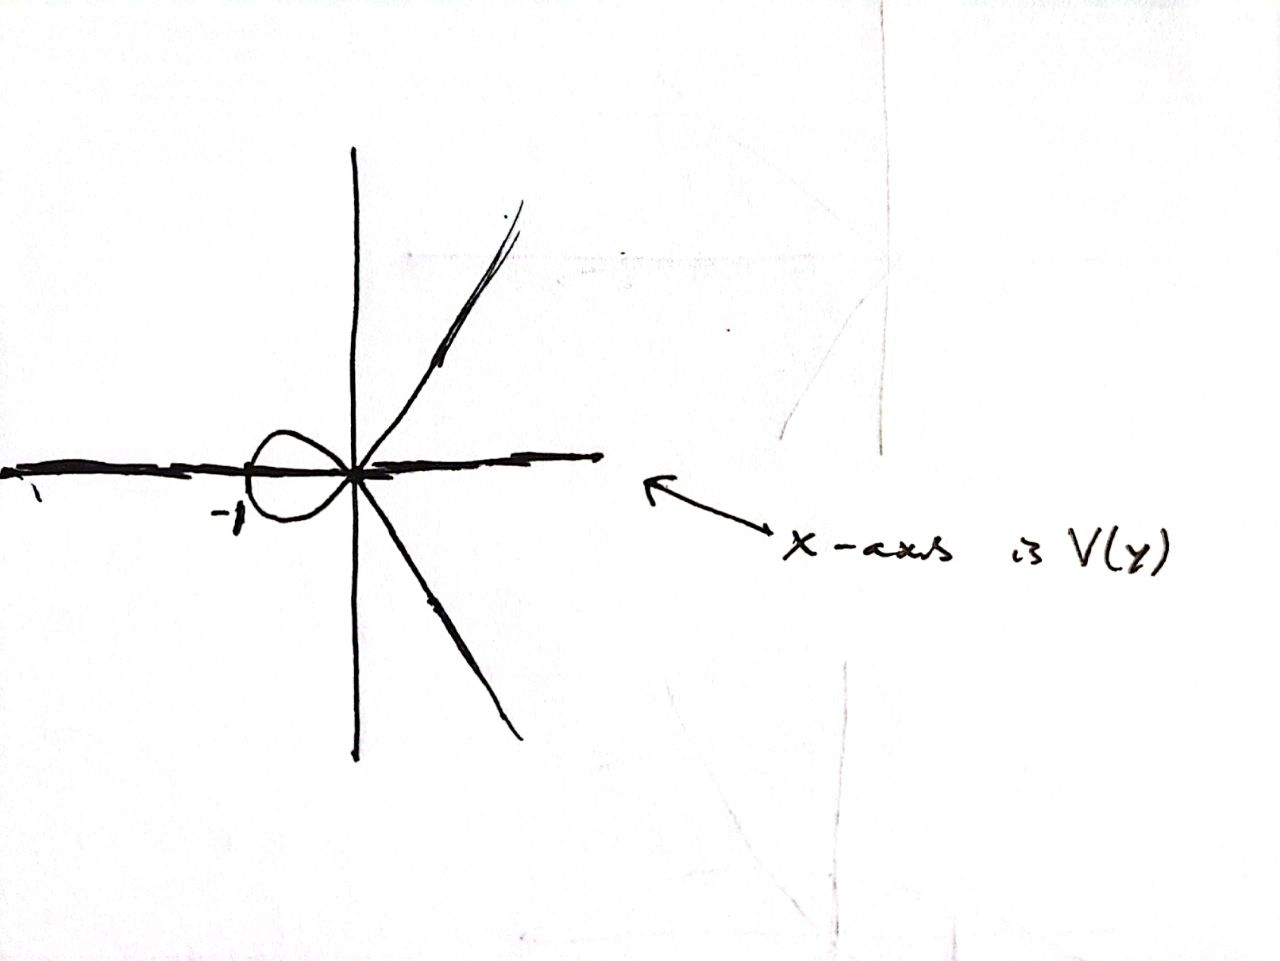
\includegraphics[width=0.5\textwidth]{2d.jpg}
        \label{fig:2d-jpg}
    \end{figure}

    We have $Y \cap V(y) = \left\{ -1,0 \right\} $. Now $\varphi^{-1}(V(y))$ is
    precisely the points that map onto $Y \cap V(y) = \left\{ -1,0 \right\} $,
    and we thus see that as $t$ traverses $\mathbb{R}$,
    $\varphi(t)$ traverses the graph depicted, $Y$, starting from the bottom.
    The first time it attains the value $0$ thus corresponds to $t = -1$, then
    it completes a half-circle and attains the value $-1$ at $t=0$, whereafter
    it completes another half-circle and attains the value $0$ again at $t=1$.
    These are the only times $\varphi(t), t \in \mathbb{C}$ attains values on
    $Y \cap V(y) = \left\{ (x,0)  \colon x \in \mathbb{R} \right\} $.\\
    \linebreak
    \textbf{3:} Since $X \subset \mathbb{A}^{n}$ is an algebraic set, there
    exist polynomials $f_1, \ldots, f_s \in  k\left[ x_1 , \ldots , x_n \right] $ such that
    $X = V\left( f_1, \ldots, f_s \right) $ by Hilbert's basis theorem;
    similarly, there exist $g_1, \ldots, g_r \in k\left[ x_1, \ldots, x_m \right] $ 
    such that
    $Y = V\left( g_1, \ldots, g_r \right) $ by Hilbert's basis theorem.\\
    \linebreak
    Now we can consider each $f_i$ and $g_i$ as a function on
    $k\left[ x_1, \ldots, x_{n+m} \right] $ by letting
    $\tilde{f_i} (x_1, \ldots, x_{n+m}) = f_i (x_1, \ldots, x_n)$ and
    $\tilde{g_i} \left( x_1, \ldots, x_{n+m} \right) =
    g_i \left( x_{n+1}, \ldots, x_{n+m} \right) $. We then claim that
    \[
    X \times Y = V\left(\tilde{f_1}, \ldots, \tilde{f_s},
    \tilde{g_1}, \ldots, \tilde{g_r} \right) .
    \] 
    $\left( \subset  \right) $ : Let $ (x,y) = (x_1, \ldots, x_n, y_1, \ldots, y_m) \in
    X \times Y$. Then
    for each $\tilde{f_i}$, we have $\tilde{f_i}(x,y) = f_i (x)
    = 0$ and for each $g_i$, we have
    $\tilde{g_i}(x,y) = g_i (y) = 0$.\\
    \linebreak
    $\left( \supset \right) $ : Let $(x,y) = (x_1, \ldots, x_n, y_1, \ldots,
    y_m) \in V \left( \tilde{f_1}, \ldots, \tilde{f_s}, \tilde{g_1},
    \ldots, \tilde{g_r} \right) $. Then for all $i$ we have
    $0 = \tilde{f_i}(x,y) = f_i (x)$ and $0 = \tilde{g_i}(x,y) = g_i(y)
    $. Thus
    $x = (x_1, \ldots, x_n) \in V\left( f_1, \ldots, f_s \right) = X$ and
    $y = \left( y_1, \ldots, y_m \right) \in V(g_1, \ldots, g_r) = Y$.\\
    \linebreak
    (b) Let $T_i  \colon k\left[ x_1, \ldots, x_{n+m} \right] \to k\left[
    x \right] $ by
    $T_i \left( x_1, \ldots, x_{n+m} \right) = x_i$.\\
    Then $T = \left( T_1, \ldots, T_n \right)  \colon k\left[ x_1, \ldots,
    x_{n+m} \right] \to k\left[ x_1, \ldots, x_n \right] $ and the projection
    $X \times Y \to X$ agree on all points of $X \times Y$ :
    $T (x_1, \ldots, x_{n+m}) = \left( x_1, \ldots, x_n \right) = pr_X \left(
    x_1,\ldots, x_{n+m} \right) $.\\
    \linebreak
    Similarly, $S = \left( T_{n+1}, \ldots, T_{n+m} \right)  \colon
    k\left[ x_1, \ldots, x_{n+m} \right] \to k\left[ x_1, \ldots, x_m \right] $ 
    agrees with the projection $X \times Y \to Y$ since
    $S \left( x_1 ,\ldots, x_{n+m} \right) =
    \left( x_{n+1}, \ldots, x_{n+m} \right) = pr_{Y}
    \left( x_1 ,\ldots, x_{n+m} \right) $ for all
    $(x_1, \ldots, x_{n+m}) \in X \times Y$. By definition, the
    projection maps $X \times Y \to X$ and $X \times Y \to Y$ are thus
    morphisms.\\
    \linebreak
    (c) Consider the projections $pr_X  \colon X\times Y \to X$ and
    $pr_Y  \colon X\times Y \to Y$. Then
    by $(b)$ these are morphisms.
    Now $X = pr_X \left( X \times Y \right) $, so
    $pr_X^{-1}(X) = X \times Y$ and since $X \times Y$ is irreducible,
    $X$ is irreducible too by the lemma on page 3 on the notes of lecture 9.\\
    Similarly, $Y = pr_Y (X\times Y)$, so 
    $pr_Y^{-1}(Y) = X \times Y$, so since $X \times Y$ is irreducible, $Y$ is
    irreducible by the same lemma.\\ 
\linebreak

 (d) Suppose $X \times Y = A \cup B$. Let $X_A =
    \left\{ p \in X  \colon p \times Y \subset A \right\} $ and
    $X_B = \left\{ p \in X  \colon p \times Y \subset B \right\} $.
    Considering the sets in the Zariski topology, we see that
    \[
    p \times Y = \left( p \times Y \cap A \right) \cup \left( p \times Y \cap B \right)
    \]
    and since each $p \times Y$ is irreducible as it is isomorphic to $Y$, each
    $p \times Y$ is contained in $A$ or $B$. Hence $X = A \cup B = X_A \cup X_B
    $. Now, for some $y \in Y$, the inclusion $X \to X \times Y$ by
    $x \to (x,y)$ is a morphism. Thus the preimages
    $\left\{ x  \colon (x,y) \in A \right\}$ are closed, and arbitrary
    intersections of closed sets are closed, so 
    $X_A = \left\{ x  \colon x \times Y \subset A \right\} = \bigcap_{y \in Y} 
    \left\{ x  \colon (x,y) \in A \right\} $ is closed and likewise for 
    $X_B$. Thus they are algebraic subsets, so $X$ is reducible,
    a contradiction.\\
    \linebreak
    


    \textbf{4:} We will show $(i) \implies (ii) \implies (iii) \implies (i)$.\\
    \linebreak
    $(i) \implies (ii)$ :\\
    If $V$ is a point, say $V = \left\{ (a_1, \ldots, a_n) \right\} $, then
    $I(V) = (x_1 - a_1, \ldots, x_n - a_n)$. Now this is the kernel of the
    evaluation function on $k\left[ x_1, \ldots, x_n \right] $ at the point
    $(a_1, \ldots, a_n)$. That is, define
    $\varphi  \colon k\left[ x_1, \ldots, x_n \right] \to k$ by
    $\varphi (f) = f(a_1, \ldots, a_n)$. Since $k \subset  k \left[ x_1,
    \ldots, x_n \right] $, this is clearly surjective, and
    $\varphi (f) = 0$ if and only if $f(a_1, \ldots, a_n) = 0$. Writing
    $g (x_1, \ldots, x_n) = f(x_1 + a_1, \ldots, x_n + a_n)$, we thus find
    $g(0, \ldots, 0) = 0$ and as the composition of polynomial functions is
    a polynomial function by a previous homework assignment, we have that
    the constant term of the polynomial $g$ is $0$. Hence
    $g \in \left( x_1, \ldots, x_n \right) $ and thus
    $f \in \left( x_1 - a_1, \ldots, x_n - a_n \right) $.
    Thus 
    \[
        k\left[ x_1, \ldots, x_n \right] / \left( x_1 - a_1, \ldots, x_n - a_n \right) 
        \cong k
    \]
    so since  $k$ is a field, $(x_1- a_1, \ldots, x_n - a_n)$ is a maximal
    ideal. In particular,
    \[
    \Gamma (V) = k\left[ x_1, \ldots, x_n \right] / I(V)
    = k\left[ x_1, \ldots, x_n \right] / (x_1 - a_1, \ldots, x_n - a_n)
    = k
    \] 
    $(ii) \implies (iii)$ : Clearly, if
    $\Gamma (V) = k$, then any point of 
    $\Gamma(V) = k$ functions as a basis. Namely, for any $f \in \Gamma(V)$, it
    corresponds to some $k_1 \in k$, and since $k = \Span (k_1)$ since $k$ is
    a field, we have that $f$ generates $\Gamma (V)$. By definition then
    $\dim_k \Gamma(V) = \dim_k k = 1 < \infty$.\\
    \linebreak
    $(iii) \implies (i)$: We may assume $k$ is algebraically closed.\\
    Since $V$ is an affine variety, we have by Hilbert's basis theorem that
    $V = V(I)$ for some ideal  $I$ of $k\left[ x_1, \ldots, x_n \right] $.\\
    Now $\dim_k \Gamma (V) = \dim_k k\left[ x_1, \ldots, x_n \right] / I(V)
    < \infty$ by assumption, so by corollary 4 in section 1.7 in Fulton,
    $V\left( I(V) \right) = V$ is a finite set of points. Since $V$ is
    a variety, it must in particular be a single point, since if 
    $V = \left\{ p_1, \ldots, p_r \right\} $ where each $p_i$ is a point, then
    $V = \left\{ p_1 \right\} \cup \ldots \cup \left\{ p_r \right\} $ and each
    $\left\{ p_i \right\} $ is a variety as it is the hypersurface of
    the evaluation function at $p_i$ in $k\left[ x_1, \ldots, x_n \right] $.\\
    \linebreak
    \textbf{5:} By problem 1.(b) in homework 3, we have that there
    is a natural bijection between radical ideals in 
    $k\left[ x_1, \ldots, x_n \right] / I(X) = \Gamma(X)$ and
    radical ideals in $k\left[ x_1, \ldots, x_n \right] $ containing
    $I(X)$. Now by corollary 1 to Hilbert's Nullstellensatz in section 1.7 in
    Fulton, we have that there is a bijective correspondence between radical
    ideals and algebraic sets of $k\left[ x_1 ,\ldots, x_n \right] $ and
    $\mathbb{A}^{n}$ given by $I(V(I)) = I$ and $V(I(V)) = V$.\\
    Now any radical ideal $R$ containing $I(X)$ corresponds to
    an algebraic set $V(R) \subset V(I(X)) = X$. And any algebraic set
    $V \subset X$ corresponds to a radical ideal $\sqrt{ I(V)} \supset I(X)$ 
    Hence
    we have a bijective correspondence between radical ideals of $k\left[ x_1
    ,\ldots, x_n \right] $ containing $I(X)$ and algebraic subsets of $X$.\\
    Composing the bijective correspondences, we thus get a bijective
    correspondence between algebraic subsets of $X$ and radical ideals in
    $\Gamma(X)$.
    
 




















\end{document}
